\documentclass[12pt,a4paper,twoside]{book}


% \usepackage[utf8]{inputenc}
\usepackage[a4paper,inner=3.5cm,outer=2.5cm]{geometry}

\usepackage[titletoc,title,toc,page]{appendix}
\usepackage{tabularx}
\usepackage{array}
\usepackage{amsmath}
\usepackage{unicode-math}

\usepackage{verbatim}
\usepackage{placeins}
\usepackage{listings}
\usepackage{hyperref}
\usepackage[english]{babel}
\usepackage{tikz}
\usepackage{parskip}

\usepackage{graphicx}
\usepackage{blindtext}
\usepackage{chngcntr}
\counterwithin{table}{chapter}

\usepackage{newlfont}
\usepackage{fancyhdr}
\usepackage{indentfirst}
% \usepackage[utf8]{inputenc}
\usepackage{float}
\usepackage{hyperref}
\usepackage[capitalize,noabbrev]{cleveref}
\usepackage{soul}
\usepackage[font=footnotesize,labelfont=bf]{caption}

\usepackage{multirow}
\usepackage{hyphenat}
\hyphenation{mate-mati-ca recu-perare}

\usepackage{lscape} 

\usepackage{natbib}
\bibliographystyle{alpha}
\setcitestyle{super,open={[},close={]}}

\newcommand{\rom}[1]{\uppercase\expandafter{\romannumeral #1\relax}}

\usepackage{pdfpages}

\begin{document}
% Per spostare i vari elementi più su o più giù gioca con i valori di vspace che ci sono tra uno e l'altro
\pagestyle{empty}
\newgeometry{
    left=20mm,
    right=20mm,
    top=20mm,
    bottom=20mm
}

\begin{titlepage}

\begin{center}

% marchio di ateneo

\includegraphics[width=6.5cm,height=4.7cm]{img/marchio-di-ateneo.png}

\vspace{10mm}

% \large is 12pt
{\large{\bf{Dipartimento di Scienze ed Ingegneria Informatica}}}

\vspace{5mm}

% \Large is 14.4pt
{\Large{\bf{Corso di Informatica}}}

\vspace{15mm}

{\Huge{\bf A Study on Applications of }}\\
\vspace{3mm}
{\Huge{\bf Homomorphic Encryption in }}\\
\vspace{3mm}
{\Huge{\bf Privacy-Preserving Protocols}} \\

\end{center}

\vspace{10mm}

\begin{minipage}[t]{0.50\textwidth}
{\large{\bf Relatore: \\ Chiar.mo Prof.\\ FEDERICO MONTORI}}

\vspace{3mm}

{\large{\bf Correlatore: \\ Chiar.mo Prof.\\ SAVERIO GIALLORENZO}}
\end{minipage}
\hfill
\begin{minipage}[t]{0.40\textwidth}\raggedleft
{\large{\bf Presentata da: \\ DIEGO BARBIERI}}
\end{minipage}

\vspace{30mm}

\rule[0.5cm]{15.8cm}{0.6mm}

\begin{center}
{\large{\bf Sessione di Luglio 2025 \\}}
{\large{\bf Anno Accademico 2024/2025\\}}
\end{center}

\end{titlepage}

\restoregeometry
\newpage

% https://tex.stackexchange.com/questions/26538/words-scattered-randomly-in-on-coverpage
\begin{tikzpicture}[overlay,remember picture,shift=(current page.center)]
\pgfmathsetseed{3}


\foreach [count=\count] \word in {Homomorphic Encryption, Privacy, Network Protocols, Zero-Trust, Location} {
\node [
    xshift={(mod(\count,3)-1)*(\paperwidth/4)},
    yshift={(mod(\count,7)-3)*(\paperwidth/6)},
    xshift=rand*4cm,
    yshift=rand*2cm,
    % rotate=rand*35,
    % opacity=rnd*0.5+0.125,
    font=\large] {\word};
}
\end{tikzpicture}
\newpage

\topmargin=6.5cm
\begin{flushright}
\emph{
\LARGE{La dedica}\\\vspace{2mm}
\LARGE{anche quella se vuoi}\\\vspace{3mm} 
\LARGE{su più righe} 
}
\end{flushright}
\newpage~\newpage
\pagenumbering{gobble}


% \newgeometry{
%     left=20mm,
%     right=20mm,
%     top=20mm,
%     bottom=20mm
% }


\chapter*{Abstract}
Abstract qui (ti consiglio di farlo alla fine)

\topmargin=-1cm
\tableofcontents
\thispagestyle{empty}
\listoftables
\thispagestyle{empty}
\listoffigures
\thispagestyle{empty}
\newpage~\newpage

\pagenumbering{arabic}
% \setcounter{chapter}{1}
\raggedbottom
\chapter{Introduction} \label{chap:intro}

\pagestyle{plain}
\setcounter{page}{1}


\chapter{Background} \label{chap:background}

This chapter will discuss the theoretical background needed to understand the protocol presented in this thesis. We will cover the main network protocols used in distributed systems, such as Request-Response and Publish-Subscribe, and how they can be applied to IoT devices. We will also discuss Universal Location Referencing, Space-Filling Curves, and Privacy-Preserving techniques, such as Homomorphic Encryption, which are the foundation of the solution proposed.

\section{Request-Response Protocol}

Request-response is a fundamental communication pattern in distributed systems where a client sends a request to a server and waits for a response. This synchronous communication model is characterized by its simplicity and direct interaction between parties, making it suitable for operations requiring immediate feedback and confirmation.

\subsection{HTTP}
HTTP (Hypertext Transfer Protocol) is the foundation of data communication on the World Wide Web. It operates as a request-response protocol, allowing clients to request resources from servers and receive responses. HTTP supports various methods (GET, POST, PUT, DELETE) for different types of operations and is extensible through headers and status codes.

\subsubsection{HTTPS}
HTTPS is a version of HTTP built on the SSL/TLS protocol, providing secure communication over a computer network. It encrypts data exchanged between clients and servers, ensuring confidentiality and integrity. HTTPS is essential for protecting sensitive information from eavesdropping and tampering.

One of the key features of HTTPS is its use of certificates to authenticate the server, ensuring that clients are communicating with the intended entity. This is possible through a relatively high usage of computational resources, which is a trade-off for the enhanced security it provides.

\subsection{Request-Response in IoT devices}
HTTPS is a commonly used choice also for IoT devices. However, its usability is often limited due to several factors:
\begin{itemize}
    \item \textbf{Resource Constraints\cite{mazhar2023iotsecurity}}: Encrypting and decrypting certificate standards (RSA, EEC, AES) can be computationally expensive, which is a significant concern for IoT devices with limited processing power and memory.
    \item \textbf{Lack of Secure Firmware Updates\cite{cyberark2024iot}}: Many IoT devices do not support secure firmware updates, making it difficult to patch vulnerabilities in the HTTPS implementation.
    \item \textbf{Weak or Nonexistent Certificate Validation\cite{bishopfox2020weakcertificates}}: Many IoT devices do not validate server certificates properly, leading to potential vulnerabilities.
\end{itemize}

This limitation has led to the development of alternative protocols and standards that are more suitable for IoT devices, such as CoAP (see \cref{sec:coap}) and MQTT (see \cref{sec:mqtt}). These protocols are designed to be lightweight and efficient, making them more suitable for resource-constrained devices.

\subsection{CoAP} \label{sec:coap}

CoAP (Constrained Application Protocol) is a specialized web transfer protocol designed for constrained devices and low-power networks\cite{rfc7252}. It operates over UDP, making it lightweight and suitable for IoT applications. CoAP supports request-response interactions similar to HTTP but is optimized for low-bandwidth and high-latency environments.

The protocol presents several key features:
\begin{itemize}
    \item Web protocol fulfilling M2M requirements in constrained
      environments.
    \item UDP-based with support for multicast.
    \item Low header overhead and parsing complexity.
    \item URI and Content-type support.
    \item Simple proxy and caching capabilities.
    \item A stateless HTTP mapping, allowing proxies to be built providing access to CoAP resources via HTTP in a uniform way or for HTTP simple interfaces to be realized alternatively over CoAP.
    \item Security binding to Datagram Transport Layer Security (DTLS)
\end{itemize}

Due to its design, CoAP can replicate the RESTful architecture of HTTP, supporting methods such as GET, POST, PUT, and DELETE. Additionally, CoAP provides an \textit{observe} mechanism that enables clients to subscribe to resources and receive notifications upon changes.

Henceforth, unless otherwise specified, any reference to an HTTP request should be interpreted as referring to a \textbf{CoAP request}.

\section{Publish-Subscribe Protocol}
Publish-Subscribe (Pub/Sub) is an asynchronous messaging pattern where senders (publishers) categorize messages into topics without the knowledge of the receivers (subscribers). Subscribers express interest in specific topics and receive messages published on those topics. This decoupled architecture enables scalable and flexible communication in distributed systems.

\subsection{MQTT} \label{sec:mqtt}
MQTT (Message Queuing Telemetry Transport) is a lightweight, open-source messaging protocol designed for constrained devices and low-bandwidth, high-latency networks. It implements the publish-subscribe pattern over TCP/IP, providing three quality service levels for message delivery and supporting various security features.

The protocol defines three main network entities:
\begin{itemize}
    \item \textbf{Message Broker}: The central component that manages message routing between publishers and subscribers. It receives messages from publishers and forwards them to subscribers based on their subscriptions.
    \item \textbf{Publisher}: A client that sends messages to the broker on specific topics. 
    \item \textbf{Subscriber}: A client that expresses interest in specific topics and receives messages published to those topics by the broker.
\end{itemize}

\subsubsection{MQTT Quality of Service Levels}

MQTT provides three quality of service (QoS) levels to ensure message delivery reliability:
\begin{itemize}
    \item \textbf{QoS 0 (At most once)}: The message is delivered at most once, with no acknowledgment from the receiver. This level is suitable for applications where occasional message loss is acceptable.
    \item \textbf{QoS 1 (At least once)}: The message is guaranteed to be delivered at least once, with acknowledgment from the receiver. This level ensures that messages are not lost but may result in duplicates.
    \item \textbf{QoS 2 (Exactly once)}: The message is guaranteed to be delivered exactly once, using a four-step handshake process. This level provides the highest reliability but incurs more overhead.
\end{itemize}

\subsubsection{MQTT Security}

As we mentioned, one of the key features of MQTT is the possibility to scale the protocol to fit the needs of the application. This is possible by using different security features, such as TLS/SSL for secure communication, authentication mechanisms to verify client identities, and access control lists to restrict topic access. These features help protect against unauthorized access and ensure the integrity of messages exchanged between clients.

\subsubsection{MQTT Workflow}

\begin{figure}[h]
    \centering
    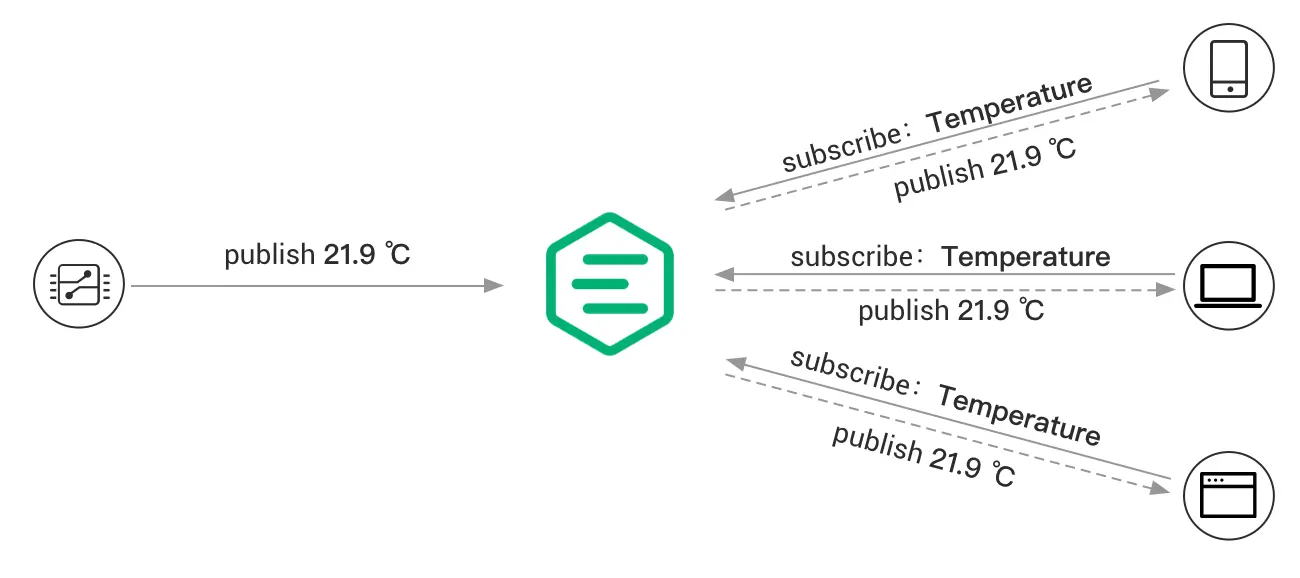
\includegraphics[width=\columnwidth]{img/mqtt-workflow-example.png}
    \caption{MQTT Workflow}
    \label{fig:mqtt-workflow}
\end{figure}

Generally, the MQTT workflow starts with the client establishing a connection to the broker, using a TCP/IP connection with optional TLS/SSL security. Once connected, the client can publish messages to specific topics or subscribe to topics of interest. The broker then routes messages to subscribers based on their subscriptions (see \cref{fig:mqtt-workflow}).

\subsection{LA-MQTT} \label{sec:la-mqtt}
LA-MQTT~\cite{montori2022lamqtt} extends the standard MQTT protocol by incorporating location-based features. It enables spatial queries and location-aware message routing, making it particularly suitable for IoT applications requiring geographical context in message distribution.

The protocol is first introduced to resolve the limitations of traditional MQTT in handling location-based data.

\begin{table}[h]
\small
\begin{tabularx}{\linewidth}{|l|X|X|X|p{4cm}|}
\hline
\textbf{API} & \textbf{Subject} & \textbf{MQTT OP} & \textbf{Topic} & \textbf{Payload} \\ \hline
Position publish & MC & Publish & GPS\_DATA & $\{position: ( P_i )\}$ \\ \hline
Topic subscription & MC & Subscribe & $C(i, t_s)$ & * \\ \cline{2-5}
 & MC & Publish & MC\_SUB & $\{ mc: i, topic: t_s \}$ \\ \hline
Geo fence publish & LDS & Publish & GEO\_FENCE\_DATA & $\{topic: t_s, content: c_s, $\newline$region: g_s, event: e_s\}$ \\ \hline
Content publish & Backend & Publish & $C(i, t_s)$ & $\{content: c_s\}$ \\ \hline
\end{tabularx}
\caption{The LA-MQTT Publish-subscribe Operations}
\label{table:la-mqtt}
\end{table}

Table \ref{table:la-mqtt} summarizes the main operations of the LA-MQTT protocol, highlighting the interactions between clients (MC), location data sources (LDS), and the backend system.

Those operations include:
\begin{itemize}
    \item \textbf{Position Publish}: MC publishes their GPS data to the broker, allowing other clients to receive updates on their positions.
    \item \textbf{Topic Subscription}: MCs subscribe to specific topics, enabling them to receive messages related to their areas of interest.
    \item \textbf{Geo fence Publish}: LDSs publish geo fence data, which includes the topic, content, region, and event associated with the Geo fence.
    \item \textbf{Content Publish}: The backend publishes content related to the subscribed topics, forwarding it to the subscribed MCs.
\end{itemize}

LA-MQTT integrates two privacy-preserving strategies within its client-side architecture:
The first strategy is based on randomized location perturbation. This method applies controlled noise to the GPS coordinates before transmission. Specifically, for a given GPS value $P_i$, a user-defined number of decimal digits is preserved, while the remaining digits are randomly replaced. This approach balances between:
\begin{itemize}
    \item Privacy Preservation (PP): Higher randomness enhances anonymity.
    \item Spatial Precision (SP): Excessive perturbation can degrade the accuracy of spatial notifications.
\end{itemize}
The second strategy involves the use of dummy updates. Here, the MC alternates between sending real and synthetic (dummy) location data. In each sequence of updates, only one is the actual position; the others are randomly generated or trajectory-based decoys.

\section{Universal Location Referencing}
Universal Location Referencing provides standardized methods for encoding and representing geographical locations. These systems ensure consistent and unambiguous location representation across different applications and platforms.

\subsection{Background: Distance Measures Between Vectors}
\label{sec:background-distances}

In many applications, especially related to positioning and spatial data, it is essential to measure the similarity or dissimilarity between vectors. This is particularly relevant in fields such as machine learning, computer vision, and geographic information systems. To analyze similarity or dissimilarity between vectors $\mathbf{x}, \mathbf{y} \in \mathbb{R}^n$, three standard distance metrics are:

\begin{description}
  \item[Cosine similarity:]
  \[
    \mathrm{CS}(\mathbf{x}, \mathbf{y}) 
    = \frac{\sum_i x_i y_i}{\|\mathbf{x}\| \cdot \|\mathbf{y}\|}.
  \]
  This measures the angle between vectors and is scale‑invariant.

  \item[Euclidean distance:]
  \[
    \mathrm{ED}(\mathbf{x}, \mathbf{y}) 
    = \sqrt{\sum_i (x_i - y_i)^2}.
  \]
  It represents the straight-line distance but involves a non-linear square root.

  \item[Manhattan distance:]
  \[
    \mathrm{MD}(\mathbf{x}, \mathbf{y}) 
    = \sum_i |x_i - y_i|.
  \]
  Also known as the $\ell_1$ norm, it sums up absolute differences.
\end{description}
\subsection{Cantor Pairing}

Cantor Pairing is a mathematical technique that uniquely maps two natural numbers to a single natural number (\cref{fig:cantor}). This bijective function $\pi: \mathbb{N} \to \mathbb{N}$ is particularly useful in computer science for combining two coordinates into a single value while maintaining the ability to recover the original coordinates.

More formally, the Cantor pairing function is defined as:
\[
    \pi(x, y) = \frac{(x + y)(x + y + 1)}{2} + y
\]

Although this function does not preserve algebraic properties, it provides some unique properties derived from the fact that it segments the two-dimensional space into a zig-zag pattern.

\[
    \pi(x, y) + 1 = \pi(x - 1, y + 1)
\]

Moreover, we also need to define the behavior of the function when one hits the boundaries of the first quadrant:

\[
    \pi(x, 0) + 1 = \pi(x + 1, 0)
\]

At last, we denote the starting point of the Cantor pairing function as \( \pi(0, 0) = 0 \). This means that the function starts at the origin of the two-dimensional space and maps it to zero in the one-dimensional space. The inverse of the Cantor pairing function can be computed as follows:
\[
    \pi^{-1}(z) = \left( \frac{n(n + 1)}{2} - z, z - \frac{n(n + 1)}{2} \right)
\]
Where \( n \) is the largest integer such that \( \frac{n(n + 1)}{2} \leq z \). This allows us to retrieve the original coordinates \( (x, y) \) from the single value \( z \).

This function is widely used in computer science, particularly in data structures and algorithms, where it is necessary to map multi-dimensional data to a single dimension for efficient storage and retrieval. It is also used in various applications such as database indexing, spatial data representation, and cryptography.


\vspace{5mm}

\begin{figure}[h]
    \centering
    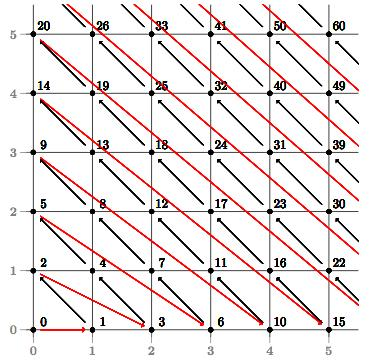
\includegraphics[width=6.5cm,height=4.7cm]{img/cantor-pairing.jpg}
    \caption{Visualization of the Cantor pairing function mapping two-dimensional coordinates to a single value}
    \label{fig:cantor}
\end{figure}

\vspace{5mm}

\section{Space Filling Curves}
Space-filling curves are mathematical curves that pass through every point in a multi-dimensional space. They provide a way to map multi-dimensional data to a single dimension while preserving spatial locality, making them valuable for spatial indexing and data organization.

The most common space-filling curves include (\cref{fig:space-filling}):
\begin{itemize}
    \item \textbf{Z-order Curve}
    \item \textbf{Hilbert Curve}
\end{itemize}

%\vspace{5mm}

\begin{figure}[h]
    \centering
    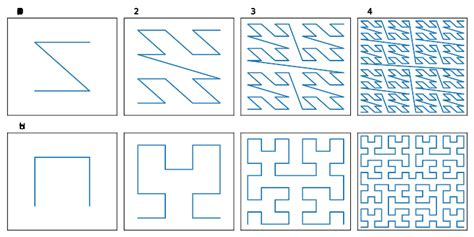
\includegraphics[width=6.5cm,height=4.7cm]{img/hilbert-z-order.jpg}
    \caption{Comparison of Z-order and Hilbert curves in two-dimensional space}
    \label{fig:space-filling}
\end{figure}

\vspace{5mm}

The Hilbert Curve is particularly notable for its ability to preserve locality, meaning that points that are close in multi-dimensional space remain close in the one-dimensional representation.

On the other hand, the Z-order Curve, preserves the order of positions in a grid-like manner, making it suitable for applications requiring efficient spatial queries. Thus, it's possible to reduce the problem of finding matching points to finding the maximum prefix of two-bit strings.

\subsection{Z-order Curve} \label{sec:z-order-curve}
As mentioned, the Z-order curve is one of the most widely used space-filling curves. It maps multi-dimensional data into a single dimension, similar to the Cantor encoding function. Conversely, it has some useful properties, when applied to spatial data, such as preserving locality and allowing efficient range queries.

\subsubsection{Z-order Encoding}

The encoding process for Z-order involves interleaving the bits of the coordinates of a point in a multi-dimensional space. For example, given a point with coordinates \( (x, y) \), the Z-order encoding can be represented as:
\[
    Z(x, y) = \sum_{i=0}^{n} (x_i \cdot 2^{2i} + y_i \cdot 2^{2i+1})
\]

Where:
\begin{itemize}
    \item \( x_i \) and \( y_i \) are the bits of the binary representation of the coordinates \( x \) and \( y \).
    \item \( n \) is the number of bits used to represent each coordinate.
\end{itemize}

The Z-order curve can also be applied to encode vectors with dimensions greater than two. In this case, the encoding process involves interleaving the bits of all coordinates in a similar manner.


\subsubsection{Z-order Decoding}
The decoding process retrieves the original coordinates from the Z-order encoded value. Given a Z-order value \( Z \), the decoding can be performed by extracting the bits corresponding to each coordinate:
\[
    x = \sum_{i=0}^{n} (Z \pmod{ 2^{2i+2} }) \cdot 2^i
\]
Where:
\begin{itemize}
    \item \( Z \pmod{ 2^{2i+2} } \) extracts the bits corresponding to the \( i \)-th coordinate.
    \item The result is then shifted and combined to reconstruct the original coordinate \( x \).
\end{itemize}

The same process can be used to find the $y$ value by de-interleaving the other bits.

\subsubsection{Z-order Querying}
Let us consider a scenario where we want to find all points within a specific range in a two-dimensional space. We define \( P \) as the set of points in the space, and we want to find all points \( p \in P \) such that:
\[
    p.x \in [x_{min}, x_{max}] \quad \text{and} \quad p.y \in [y_{min}, y_{max}]
\]

We can leverage the Z-order encoding to efficiently query this range. This is possible by calculating the order of the encoding that we want to find. 
By definition, we can represent the GPS coordinates of a point \( (x_p, y_p) \) into a point \( e_p \). This point will be represented in the space of \( n \) orders, each contained in \( \mathbb{Z}_4 \).

\subsubsection{Maximum Common Prefix Search}
A key operation in Z-order-based spatial queries is finding the maximum common prefix between two Z-order encoded values. This operation is fundamental for determining spatial relationships between points.

Given two Z-order encoded values \( Z_1 \) and \( Z_2 \), we can find the maximum common prefix by following three steps. Firstly, we convert both values to their binary representation. Then, we compare the bits from left to right, stopping at the first position where the bits differ. Finally, we extract the common prefix up to that point. The cited algorithm shows that in the worst case, the maximum common prefix can be found in \( O(n) \) time, where \( n \) is the number of bits in the Z-order encoding.

The length of the common prefix determines the size of the smallest bounding box that contains both points. This property is particularly useful for:
\begin{itemize}
    \item Finding the smallest region containing multiple points
    \item Determining if points are within a certain distance of each other
    \item Optimizing spatial range queries
\end{itemize}

For example, consider two points with Z-order encodings:
\begin{align*}
    Z_1 &= 3310_4 \\
    Z_2 &= 3312_4
\end{align*}
The maximum common prefix is \( 331_4 \), indicating that these points share the same region in the first three orders of the encoded space. We used base 4 because it's the easiest way to visualize which of the four quadrants the point belongs to, as each digit represents a quadrant in a two-dimensional space.

This prefix-based approach can be extended to handle a range of queries by:
\begin{enumerate}
    \item Encoding the query range boundaries
    \item Finding the maximum common prefix of the range
    \item Generating all possible Z-order values that share this prefix
\end{enumerate}

The efficiency of this approach comes from the fact that we can perform these operations using simple bitwise operations, making it suitable for real-time applications.


\section{Privacy Preserving Techniques}
Privacy-preserving techniques ensure the protection of sensitive information while allowing necessary computations and data processing. These methods are crucial in maintaining confidentiality in distributed systems and data analysis. For example, in the context of location-based services, privacy-preserving techniques allow for the sharing of location data without revealing exact coordinates, thus protecting user privacy.

\subsection{Homomorphic Encryption}
Homomorphic Encryption(HE) is a form of encryption that allows specific types of computations to be performed on cipher text, producing an encrypted result that, when decrypted, matches the result of operations performed on the plain text.

Let us denote \( \xi_k \) the encryption function, \( \xi_k^{-1} \) the decryption function, and \( f \) a function that can be computed on plain texts. Homomorphic Encryption satisfies the property:

\[
    \xi_k(f(x)) = f(\xi_k(x))
\]

In recent years, several Homomorphic Encryption schemes have been proposed, each with different properties and capabilities. The scheme used in this thesis is the Brakerski-Gentry-Vaikuntanathan (BGV, 2011) scheme \cite{Brakerski2012-wj}, which is a leveled fully homomorphic encryption scheme that supports both addition and multiplication operations on encrypted data. The BGV scheme is particularly notable for its efficiency and ability to handle large integers, making it suitable for practical applications in privacy-preserving computations.
This scheme was based on the security of \textbf{(Ring) Learning With Errors} (RLWE) (see \cref{sec:rlwe}) problem, which is a hard problem in lattice-based cryptography. The need for such a scheme arises from the increasing demand for secure computations in various fields, including cloud computing, data analysis, and machine learning. This type of new technology is designed to resist quantum computers and cryptanalysis. 

\subsubsection{Security foundation: (Ring) Learning With Errors (RLWE)} \label{sec:rlwe}

The security of lattice-based FHE schemes, especially BGV, rests on the hardness of the Ring Learning With Errors (RLWE) problem, a ring-based variant of the Learning With Errors (LWE) problem introduced by Lyubashevsky, Peikert, and Regev in 2010 \cite{Lyubashevsky2010-jo}.
In RLWE, one works over a polynomial ring modulo both a prime $q$ and an irreducible polynomial $a(x)$:

\[
    a(x) = a_0 + a_1 x + \ldots + a_{n-1} x^{n-1}, \text{where } a_i \in \mathbb{Z}_q
\]

Samples are of the form $(a(x),\,b(x)=a(x)s(x)+e(x))$, where $e(x)$ is a small “error” polynomial. Recovering $s(x)$ given many such samples is presumed hard, based on reductions to the Shortest Vector Problem (SVP) in ideal lattices.

\subsection{Homomorphic Encryption Types}

\textbf{Fully Homomorphic Encryption (FHE)} allows the evaluation of arbitrary circuits of additions and multiplications over encrypted data, without decryption. However, earlier FHE schemes suffered from inefficiencies, particularly due to the large growth of noise. The BGV scheme answered these challenges by avoiding Gentry’s “bootstrapping” \cite{brakerski2011leveled} step via \emph{leveled} evaluation, and controlling noise through \emph{modulus switching} and \emph{relinearization} techniques.

\textbf{Partially Homomorphic Encryption (PHE)} supports only one type of operation—either addition (e.g., Paillier) or multiplication (e.g., RSA variants). These are faster than FHE but limited in expressiveness, making them suitable for simpler tasks where only one operation type is required.

\subsection{HE Translation Key} \label{sec:translation-key}

Originally introduced in 1998, Blaze, Bleumer, and Strauss (BBS)\cite{Blaze1998-cw} proposed an application called atomic proxy re-encryption, the mechanism enables ciphertexts encrypted under one public key to be transformed into ciphertexts decryptable under another key—without exposing the underlying plaintexts or private keys. It addresses the challenge of heterogeneity in multi‑actor systems, eliminating the need for a central trusted broker to perform decryption and re‑encryption. Instead, each data owner can generate a *Translation Key* that authorizes on‑the‑fly ciphertext conversion by other parties.

Consider a privacy‑preserving workflow involving three participants—Alice, Bob, and Charlie—each with their respective keypairs $(k_A^+, k_A^-)$, $(k_B^+, k_B^-)$, and $(k_C^+, k_C^-)$. Suppose Alice wants to store encrypted data on Bob’s untrusted server. She encrypts her data under $k_A^+$ and uploads the ciphertext. Since Bob cannot decrypt (he lacks $k_A^-$), Charlie would also be unable to access the data directly. However, if Alice generates and distributes a Translation Key $k_{A\to C}$, Charlie can convert the ciphertext into one encrypted under $k_C^+$ and then decrypt it with $k_C^-$, without learning Alice’s private key or Bob’s data.

The Translation Key creation requires Alice's Private key and Charlie's Public key, ensuring that only authorized parties can perform the conversion.

\[
    k_{A\to C} = f(k_A^-,k_C^+)
\]

By allowing secure key-conditional ciphertext conversion, the Translation Key mechanism preserves confidentiality across distinct encryption domains. This is particularly valuable when multiple data owners—with different keys—need to perform joint encrypted computations on a shared ciphertext under a common key.


\section{Usage of HE for Matching}
Homomorphic Encryption can be used to securely match location. To archive this, we can use different techniques such as:
\begin{itemize}
    \item \textbf{Distance Calculation}: It is archived by tweaking the distance calculation algorithms (mentioned before in \cref{sec:background-distances} e.g., Euclidean distance, Cosine similarity, Manhattan Distance) to work with encrypted coordinates. The main limit comes with the constraint that the operations must be compatible with the encryption scheme used. For instance, calculating the square Euclidean distance between two points \( (x_1, y_1) \) and \( (x_2, y_2) \) can be expressed as:
    \[
        d^2 = (x_1 - x_2)^2 + (y_1 - y_2)^2
    \]
    That can be computed homomorphically and then decrypted before computing the square root to get the actual distance. We will further discuss this in the Testing Section \ref{sec:testing-performance}.
    \item \textbf{Encoding Coordinates}: By encoding coordinates into a grid-like structure, we can reduce the problem into finding two different points sharing the same area-encoding. This approach comes with some limitations, mainly related to the precision of the approximation and the size of the grid. Still, it allows for efficient matching of points within a specific area without revealing their exact coordinates. This is done by applying a space-filling curve, such as Z-order (\cref{sec:z-order-curve}), to the coordinates.
\end{itemize}

\subsubsection{Privacy-Preserving Z-order Queries} \label{sec:privacy-preserving-z-order}

When implementing privacy-preserving location queries using Z-order encoding, we can employ homomorphic encryption to protect sensitive location data \cite{zhang2020privacy}. Let us consider a scenario where a user \( A \) wants to share their location with user \( B \) while maintaining privacy:

\begin{itemize}
    \item Let \( QK_A \) be the QuadKey representation of \( A \)'s location
    \item Let \( M_B \) be the bit mask specified by \( A \) for user \( B \)
    \item The service provider (SP) performs homomorphic multiplication: \( QK_A \otimes M_B \)
\end{itemize}

To ensure unambiguous results, we increment each value in \( qk_i \in QK_A \) by one before encryption, such that \( qk_i \in \{1,2,3,4\} \). In this scheme \cite{zhang2020privacy}:
\begin{itemize}
    \item A bitmask value of 1 preserves the location data
    \item A bitmask value of 0 masks the location data
\end{itemize}

After decryption on the client device, we:
\begin{enumerate}
    \item Remove any zero values
    \item Convert the elements back to \( \mathbb{Z}_4 \)
    \item Generate a masked QuadKey string that produces a bounding box with the desired level of detail
\end{enumerate}

This approach is computationally efficient as it requires only one round of homomorphic multiplication. The resulting bounding box effectively hides both precise locations and movement patterns, providing privacy even against colluding users.

For example, given a precise GPS coordinate \( (43.084451, -77.680069) \), the system can generate bounding boxes of varying sizes based on the privacy preferences (where the distance \( d \) represents the level of detail). This ensures that location data is shared at an appropriate granularity while maintaining user privacy.

% TODO: add other type of queries

\subsection{PHE and FHE Implications}

The choice between Partially and Fully Homomorphic Encryption has significant implications for system performance, security, and functionality. As previously discussed, the two methods used for proximity checks in a location-based scenario require careful consideration of the encryption scheme.

If the requirements only involve checking whether two positions share a common area, leveraging the speed and simplicity of the Z-order approach is recommended. This method allows the usage of PHE to perform fast proximity checks without significant overhead. As we have seen in \cref{sec:privacy-preserving-z-order}, this approach can efficiently determine if two points are within the same area by subtracting their Z-order encodings.

Conversely, if the goal is to compute a precise floating-point distance value, a homomorphically encrypted distance function (e.g., Euclidean distance) may be necessary (see \cref{lst:distance-computation-tricks}). However, it is important to note that in this case, the final result may be affected by computational noise inherent to FHE operations. Additionally, not all FHE schemes support floating-point operations directly, which can complicate the implementation because of the need to convert between integer and floating-point representations.

To conclude, the choice between PHE and FHE depends on the specific requirements of the application. One of the main advantages of PHE is its speed and simplicity, even though it is limited to a single operation type. On the other hand, FHE provides greater flexibility and expressiveness, allowing for complex computations on encrypted data. However, it comes with increased computational overhead and potential noise issues, that cannot be ignored in a production-ready system.



\chapter{System Architecture} \label{chap:system-architecture}

In this chapter, we present the system architecture for the proposed privacy-preserving location-matching protocol. The main idea is to apply the principles of homomorphic encryption to location-based services, allowing clients to securely publish and perform queries using their positions without revealing sensitive information.

\section{Use Case}
To clearly understand the system operations, let's first analyze the use case of a client who wants to find the closest parking spot available. The client needs to compute the distances between its position and the parking spots, and finally decide whether to park or not and where.

Even though it seems a straightforward mechanism, if we want to move the operations to the server, in order to preserve computational resources on the client side, a lot of challenges arise. The first one is to securely share the position of the client with the server, without exposing it to the workers. The second one is not to leak sensible information about the clients after the computation is finished.

In this scenario, it's not enough to simply encrypt the positions of the clients, as the workers need to compute the distances between the positions of the clients and the parking spots, which are also encrypted with a different key. To resolve this problem, we could just leave the parking position in clear text on the database, but this would expose the parking spots to the workers, who could then leak the information for profit. Thus, by selling the parking spots to third parties, they could be compromising the privacy of the system. In order to avoid this, and also achieve a full privacy-oriented protocol, we need to use a re-encryption mechanism, that allows the workers to compute the distances between the positions of the clients and the parking spots, without revealing the positions of the clients to the workers.

The distance problem is avoided by using the Z-order encoding, which allows us to reduce the problem of finding matching points to finding the maximum prefix of two-bit strings. In our use case, the simulated server will perform a simple encrypted subtraction between the positions of the clients and the parking spots. At last, only the client will be able to decrypt the result, which is a simple integer value that represents the distance between the two points (If the value is 0 is a perfect match). The client can then use this value to decide whether to park or not, and where. 

\section{System Overview}
The protocol is designed to combine a standard request-response protocol with a publish-subscribe mechanism.


\begin{figure}[h]
    \centering
    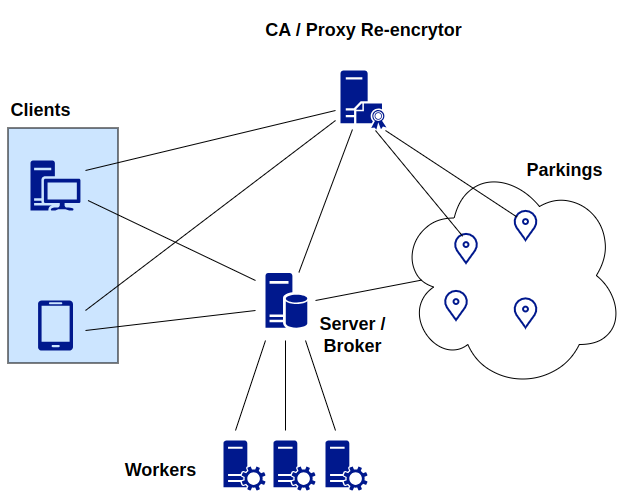
\includegraphics[width=8.5cm,height=5.5cm]{img/architecture-scheme.png}
    \caption{Visualization of the system architecture for the proposed privacy-preserving location matching protocol.}
    \label{fig:architecture}
\end{figure}

Homomorphic encryption incurs high computational costs, so the system optimizes performance by splitting the workload: the server handles only essential data processing, while workers compute the distances between client positions. Since HE allows computations on encrypted data, this approach preserves the privacy of clients' locations without compromising efficiency.

\section{Actors}

\subsection{Location Data Source}
The Location Data Sources (LDS), commonly referred to as sensors or parkings, are responsible for collecting and publishing location data. In our system, we assume they independently publish their data to the server, based on the event they register. For instance, if a sensor detects a free parking spot, it publishes the information to the broker, which will start the encryption protocol. This happens also when a parking spot is occupied, allowing the system to keep track of the available parking spots in real time.

Note that by maintaining the availability of the parking spots, independent from the clients, we can ensure that the system can provide privacy-preserving updates to the server. Conversely, if the clients were also responsible for reserving the parking spots, they would need to expose their positions to the server, which would compromise the privacy of the system.

\subsection{Mobile Clients}
MCs or Mobile Clients are the users of the system. Their main interest is to receive updates on the closest available parking spots, based on their current position. 

In our system, the client's responsibilities are very limited, as they do not trust the server and all the other actors involved in the protocol. They only need to publish their encrypted position to the server, wait for the computation to finish, and then receive the results.

\subsection{Server}
The Backend Server (commonly called Information Broker) is the central component of the system, responsible for managing the communication between clients and sensors. It also acts like a database, handling and storing the encrypted parking spot data.

This centralized component is crucial in the architecture, as it allows all sorts of mobile actors (including clients and LDs) to have a persistent connection with the system, although it's not enough if we want to achieve a full zero-trust protocol.

Thanks to HE, the server can perform computation without knowing the clear text positions of the other actors.

The second name "Information Broker" comes from the fact that the server acts like an MQTT broker, allowing clients to subscribe to topics and receive updates on the parking spots \cref{fig:architecture}. In order to create consistent and reliable communication between these two entities, without flooding the network with TCP/IP packets, the server uses a pub/sub mechanism, where the clients subscribe to a topic and the server publishes updates to that topic.

\subsection{Certification Authority / Proxy}
The certification authority (CA) is a trusted entity responsible for storing the public keys of the clients and managing the public/private keys of the parking spots. Because he is a trusted entity, the CA knows the private keys of the parking spots. In addition, it can generate the symmetric translation keys (see \cref{sec:translation-key}) required for secure computation of the client distances without revealing clear text positions.

In our system, the CA also acts like a proxy re-encryptor\cite{POLYAKOV2017FastPRE}, as it is responsible for managing the right keys for the homomorphic operation made on the encrypted data. 

\subsection{Worker}
The name Worker refers to a generic computational unit of the system, that can handle tasks from the server rewarded with a digital currency. In our case, the workers are responsible for computing the distances between the positions of the clients and the parking spots, using the homomorphic encryption scheme. 

The workers' digital reward can be described as a token that allows them to request tasks from the server. In this way, each client can act as a worker, contributing to the overall computation of the system.

\section{Network Protocol and Communication}
\subsection{Usage of different network protocols}

The MQTT protocol is used for the communication between the clients and the server. It is necessary to use a pub/sub mechanism in order to keep alive the connection between the two entities. This is achieved by having the client subscribe to a topic, while the proxy publishes updates to that topic.

Moreover, the server is responsible for managing the connection with the LDs, allowing the clients to receive updates on the parking spots. In this way, the client $MC_i$ \textbf{publishes} its position $Area_j$ to the topic $ID_{MC_i}$. The server can then apply the homomorphic operations on the data, using the keys provided by the CA.

When the computation is finished, the broker publishes the results to the topic $ID_{MC_i}$, allowing the client to receive updates on the parking spots. The client can then \textbf{subscribe} to the topic $ID_{MC_i}$ to receive updates on the parking spots.

The HTTP protocol is used for the communication between the CA and the other entities of the system. Because the CA performs atomic actions, such as key generation and translation, it is necessary to use a request-response protocol to ensure that the operations are performed in a secure and reliable way.

%\newpage

\section{Protocol Overview}
The system is designed to allow the following operations:

\begin{table}[h]
\renewcommand{\arraystretch}{1.3}
\small
\begin{tabularx}{\linewidth}{|l|X|X|X|p{4cm}|}
\hline
\textbf{API} & \textbf{Subject} & \textbf{Protocol} & \textbf{Receiver} & \textbf{Payload} \\ \hline

Position Encoding Parameters & Clients / LDs & HTTP GET & Server & - \\ \hline

Key Obtain & LDs & HTTP GET & CA / Proxy & $\{id: ID_{park_j}\}$ \\ \hline

Key Share & Client & HTTP POST & CA / Proxy & $\{id: ID_{mc},\ \text{pub. key: } k_{mc}^+\}$ \\ \hline

Position Publish & Client & MQTT PUB & Server & $\{position: \xi_{mc}(P_i)\}$ \\ \hline

Topic Subscription & Client & MQTT SUB & Server & $\{topics: [position, distance]\}$ \\ \hline

Location Publish & LDs & HTTP POST & Server & $\{\xi_{park_j}(P_j),\ id: ID_{park_j},\ \text{status} \in \{\text{free}, \text{occ.}\}\}$ \\ \hline

Translate Locations & Server & HTTP GET & CA / Proxy & $\{positions: [\xi_{park_j}(P_{j})]\}$ \\ \hline

Work Request & Worker & HTTP GET & Server & - \\ \hline

Task Finished & Worker & HTTP POST & Server & $\{worker: w_i,\ task: t_j,\ result: \xi_{park_j \to mc_i}(R)\}$ \\ \hline

Distance Publish & Server & MQTT PUB & Client & $\{distances: [\forall j \in P,\ \xi_{mc_i}(R)]\}$ \\ \hline

\end{tabularx}
\caption{System Operations Aligned with Architecture}
\label{table:system-operations}
\end{table}

\section{Distance Preference}

As we mentioned in \cref{table:system-operations}, the first operation that both the MCs and LDs need to perform is to obtain the position encoding parameters from the server. In this section, we will analyze why this is necessary and how it works.

The necessity of translating a GPS reference into a grid position encoding comes with some limitations. First of all, the grid-like structure requires a fixed size for both the whole area and the single grid cell. This operation is performed by the server, in order to ensure consistency across the whole system. This operation could be performed also by single actors, but only if they are aware of a standardized measurement unit. Moreover, the subscribers could be interested in creating a custom grid, like a system some orders of magnitude larger than the others, that should still maintain the original atomic cell size.

For our study case, we will assume that the centralized server is responsible for managing the parameters. In this way, he can generate a grid that contains the geographical area of Bologna, Italy, where the simulated parking spots are located.

% \newpage
\section{Scenario}


\begin{figure}[h]
    \centering
    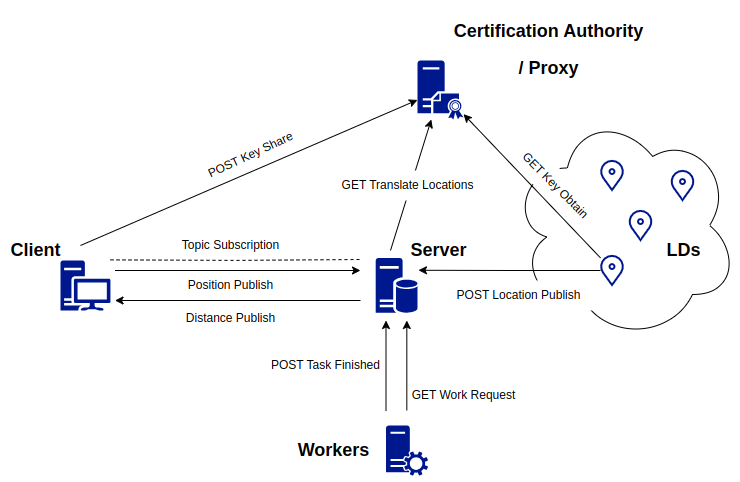
\includegraphics[width=12cm,height=7.5cm]{img/workflow.png}
    \caption{Visualization of the protocol flow}
    \label{fig:protocol-flow}
\end{figure}

\subsection{Protocol Flow}

We can summarize the protocol flow in the following steps as shown in \cref{fig:protocol-flow}:

\begin{enumerate}
    \item The clients and the parking spots register to the system, after that they receive the general position encoding parameter from the server using the \textbf{Position Encoding Parameters} API via HTTP GET request. The parameters are used to encode the positions of the clients and the parking spots. \emph{(API: \texttt{Position Encoding Parameters}, Payload: \{None\} $\to \{encoding\_params: [\text{z-order}, \text{precision}, \text{working area}, \text{grid cell size}]\}$})
    \item The mobile client $MC_i$ generates a new public/private key pair $(k_{mc_i}^+, k_{mc_i}^-)$ and sends the public key to the certification authority (CA) using the \textbf{Key Share} API via an HTTP POST request. \emph{(API: \texttt{Key Share}, Payload: $\{id: ID_{mc_i},\ k_{mc_i}^+\} \to { \text{None} }$)}
    \item After the CA verifies the client, it generates a symmetric key $k_{mc_i, park_j}$ for each parking spot $park_j$. The operation of key generation is performed by \emph{Key Translation}$(pp, k_{mc_i}^+, k_{park_j}^-)$, where $pp$ is the public parameters of the system, $k_{mc_i}^+$ is the public key of the client, and $k_{park_j}^-$ is the private key of the parking spot. Note that the translation operation must be done each time a new parking spot is added to the system.
    \item The $MC_i$ establishes an MQTT connection with the server and subscribes to the topic $ID_{MC_i}$, which is used to receive updates on the parking spots. This is done using the \textbf{Topic Subscription} API via MQTT. \emph{(API: \texttt{Topic Subscription}, Payload: $\{topics: [position, distance]\}$)}
    \item The client will then send the encrypted position $\xi_{mc}(P_i)$ to the server, where $P_i$ is the encoded position of the client. The encryption is done using the public key $k_{mc_i}^+$, ensuring that only the client can decrypt the position. This is done using the \textbf{Position Publish} \emph{(API: \texttt{Position Publish}, Payload: $\{position: \xi_{mc}(P_i)\}$)}. Moreover, this operation allows the client to also subscribe to the topic $ID_{MC_i}$, which is used to receive updates on the parking spots.
    \item The server receives the location, is notified about the MQTT subscription, and starts the translation process, by invoking the \textbf{Translate Locations} API via HTTP GET request to the CA. The CA then re-encrypts the position for each parking spot using the associated key $k_{park_j \to mc_i}$, creating the re-encrypted blob $[\forall j \in \text{P},\ \xi_{mc_i}(P_j)]$. \emph{(API: \texttt{Translate Locations}, Payload: $\{positions: [\xi_{park_j}(P_j)]\}$)}
    \item The server will then spread the re-encrypted positions to the workers, by invoking the \textbf{Work Request} API via HTTP GET request. The workers will then compute the distances between the client position and the parking spots, using the re-encrypted positions. \emph{(API: \texttt{Work Request}, $Payload: \{ worker: w_i \} \to \{task: t_j \} $})
    \item Once the workers compute the distances (or other metrics) between the client and parking spots, they send the result back using the \textbf{Task Finished} API via HTTP POST request. The result is a re-encrypted blob containing the distances between the client position and the parking spots. \emph{(API: \texttt{Task Finished}, Payload: $\{worker: w_i,\ task: t_j,\ result: \xi_{park_j \to mc_i}(R)\}$)}
    \item The server then publishes the aggregated results to the client via MQTT using the \textbf{Distance Publish} API. The payload contains the distances between the client's position and the parking spots, re-encrypted with the client's public key. \emph{(API: \texttt{Distance Publish}, Payload: $\{distances: [\forall j \in P,\ \xi_{mc_i}(R)]\}$)}
    \item Finally, the client receives the re-encrypted results from the topic subscription, decrypts them using its private key $k_{mc_i}^-$, and checks whether the location satisfies the area matching condition.
\end{enumerate}

\section{Security Considerations}

The main goal of the study is to provide a privacy-preserving location-matching protocol, that allows clients to securely publish and query their positions without revealing sensitive information. In order to fulfill this goal, we need to ensure that the system is attack-resistant and that the privacy of the clients is preserved.

In the earlier approach \cite{genova2024helamqtt}, the position-matching protocol used Euclidean distance calculations between client locations and parking spots provided by a trusted CA. While the server could not directly access this data, the mechanism inadvertently exposed the positions of mobile clients (MCs). The vulnerability stemmed from the lack of client authentication, enabling malicious actors to impersonate legitimate clients and intercept traffic. An attacker could exploit this by conducting a binary search on the client’s location, sending iterative queries based on subscribed topics. By progressively refining the search area, the attacker could pinpoint the client’s exact position, violating location privacy.

This showcased that HE is secure if and only if the encryption and decryption operation are performed correctly, preferably by the client itself.

As we also mentioned in the previous attack, the system is vulnerable to a lack of authentication of the clients. Moreover, if an attacker was able to read the network traffic, he could also manipulate the communication in order to interfere with the pub/sub mechanism.

In my implementation, I addressed those issues by introducing different techniques from the state of the art, such as using a proxy re-encryptor and a position encoding mechanism based on Z-order. The choice of leaving the decryption operation to the client ensures that no one is able to read the sensitive data, despite an increase of computational resources required to re-encrypt each position for each parking spot.

\subsection{Threat Model} \label{subsec:threatmodel}

In this section, we will analyze the threat model of the system, identifying the potential attackers and their capabilities. 


\subsection{Mitigation Strategies Malicious Actors}

\begin{table}[h]
\renewcommand{\arraystretch}{1.3}
\small
\begin{tabularx}{\linewidth}{|l|X|X|}
\hline
\textbf{Adversary} & \textbf{Goal / Attack} & \textbf{Mitigation Strategy} \\ \hline

Malicious Client &
Impersonate another client or send fake position updates. &
Use digital signatures: at the time of authentication with the CA, the client signs a digital contract that ensures that he is the one trying to access the system. \\ \hline

Malicious Worker &
Manipulate computation results or leak client-sensitive data. &
Because the user has no way of finding out if the information has been manipulated during the homomorphic phase, the server needs to implement a mechanism of \emph{fake workload} to test workers' reliability. \\ \hline

Malicious Server &
Access or manipulate sensitive client data or computational outcomes. &
Because the server could only drop the communication or modify packets, but not leak sensitive information. It's suggested to have multiple backup servers independent of one from the other. \\ \hline

Network Attacker &
Intercept and read client-sensitive data from network traffic. &
All the traffic is HE encrypted. \\ \hline

\end{tabularx}
\caption{Adversarial Threats and Mitigation Strategies}
\label{table:adversaries}
\end{table}

In the \cref{table:adversaries}, we summarize the potential adversaries and their goals, along with the mitigation strategies that can be employed to counteract their attacks. It's also important to notice that one of the assumptions of the system was that the CA is a trusted entity, moreover if an attacker is able to compromise the CA, he can also compromise the whole system. Thus, it's not worth to consider the CA as an adversary.


\definecolor{dkgreen}{rgb}{0,0.6,0}
\definecolor{gray}{rgb}{0.5,0.5,0.5}
\definecolor{mauve}{rgb}{0.58,0,0.82}

\chapter{Testing}
\section{Testing Methodology}

For the testing of the protocol, we implemented a proof-of-concept in Python, using the OpenFHE library\cite{openFHE}. The testing methodology consists of the following steps. Firstly, we generate a set of random positions for the parking spots. After that, we generate a random position for the client, we compute the z-order encoding for both the client and the parking spots, and finally we computed the distances between the client position and the parking spots using the homomorphic encryption scheme.

To ensure a fair comparison, we test different scenarios with different sets of hyper parameters, such as the number of parking spots, the number of clients running simultaneously, a range of network delays, and the edge size in meters of a grid cell (used to encode the GPS coordinates). The goal is to measure the performance of the homomorphic encryption scheme in terms of encryption and decryption time, as well as the time taken to compute the distances between the client position and the parking spots.

At the same time, we also computed the distance calculation using a clear computation (trusted backend) with encrypted with asymmetric encryption (RSA) traffic. This allows us to compare the performance of the homomorphic encryption scheme against a traditional asymmetric encryption scheme.

The testing environment consists of a virtual machine instance on a server, with the following specifications:
\begin{itemize}
    \item CPU: Intel(R) Xeon(R) Silver 4110 CPU @ 2.10GHz 16 cores
    \item RAM: 64 GB
    \item OS: Debian 11
    \item Python version: 3.8
    \item OpenFHE version: 1.3.0.0.20.4
    \item numpy version: 1.24.0
\end{itemize}

\section{Performance Evaluation} \label{sec:testing-performance}

The first test that we perform is to measure the time taken to encrypt and decrypt the client position using the homomorphic encryption scheme. The results are shown in Figure \ref{fig:testing-enc}. The time taken to encrypt around 50 parkings with the same key is around 0.5 seconds, while the time taken to decrypt the client position is around 0.2 seconds. This resoults that the homomorphic encryption scheme is efficient for this use case, but it still grows linearly with the number of data points.

\begin{figure}[h]
    \centering
    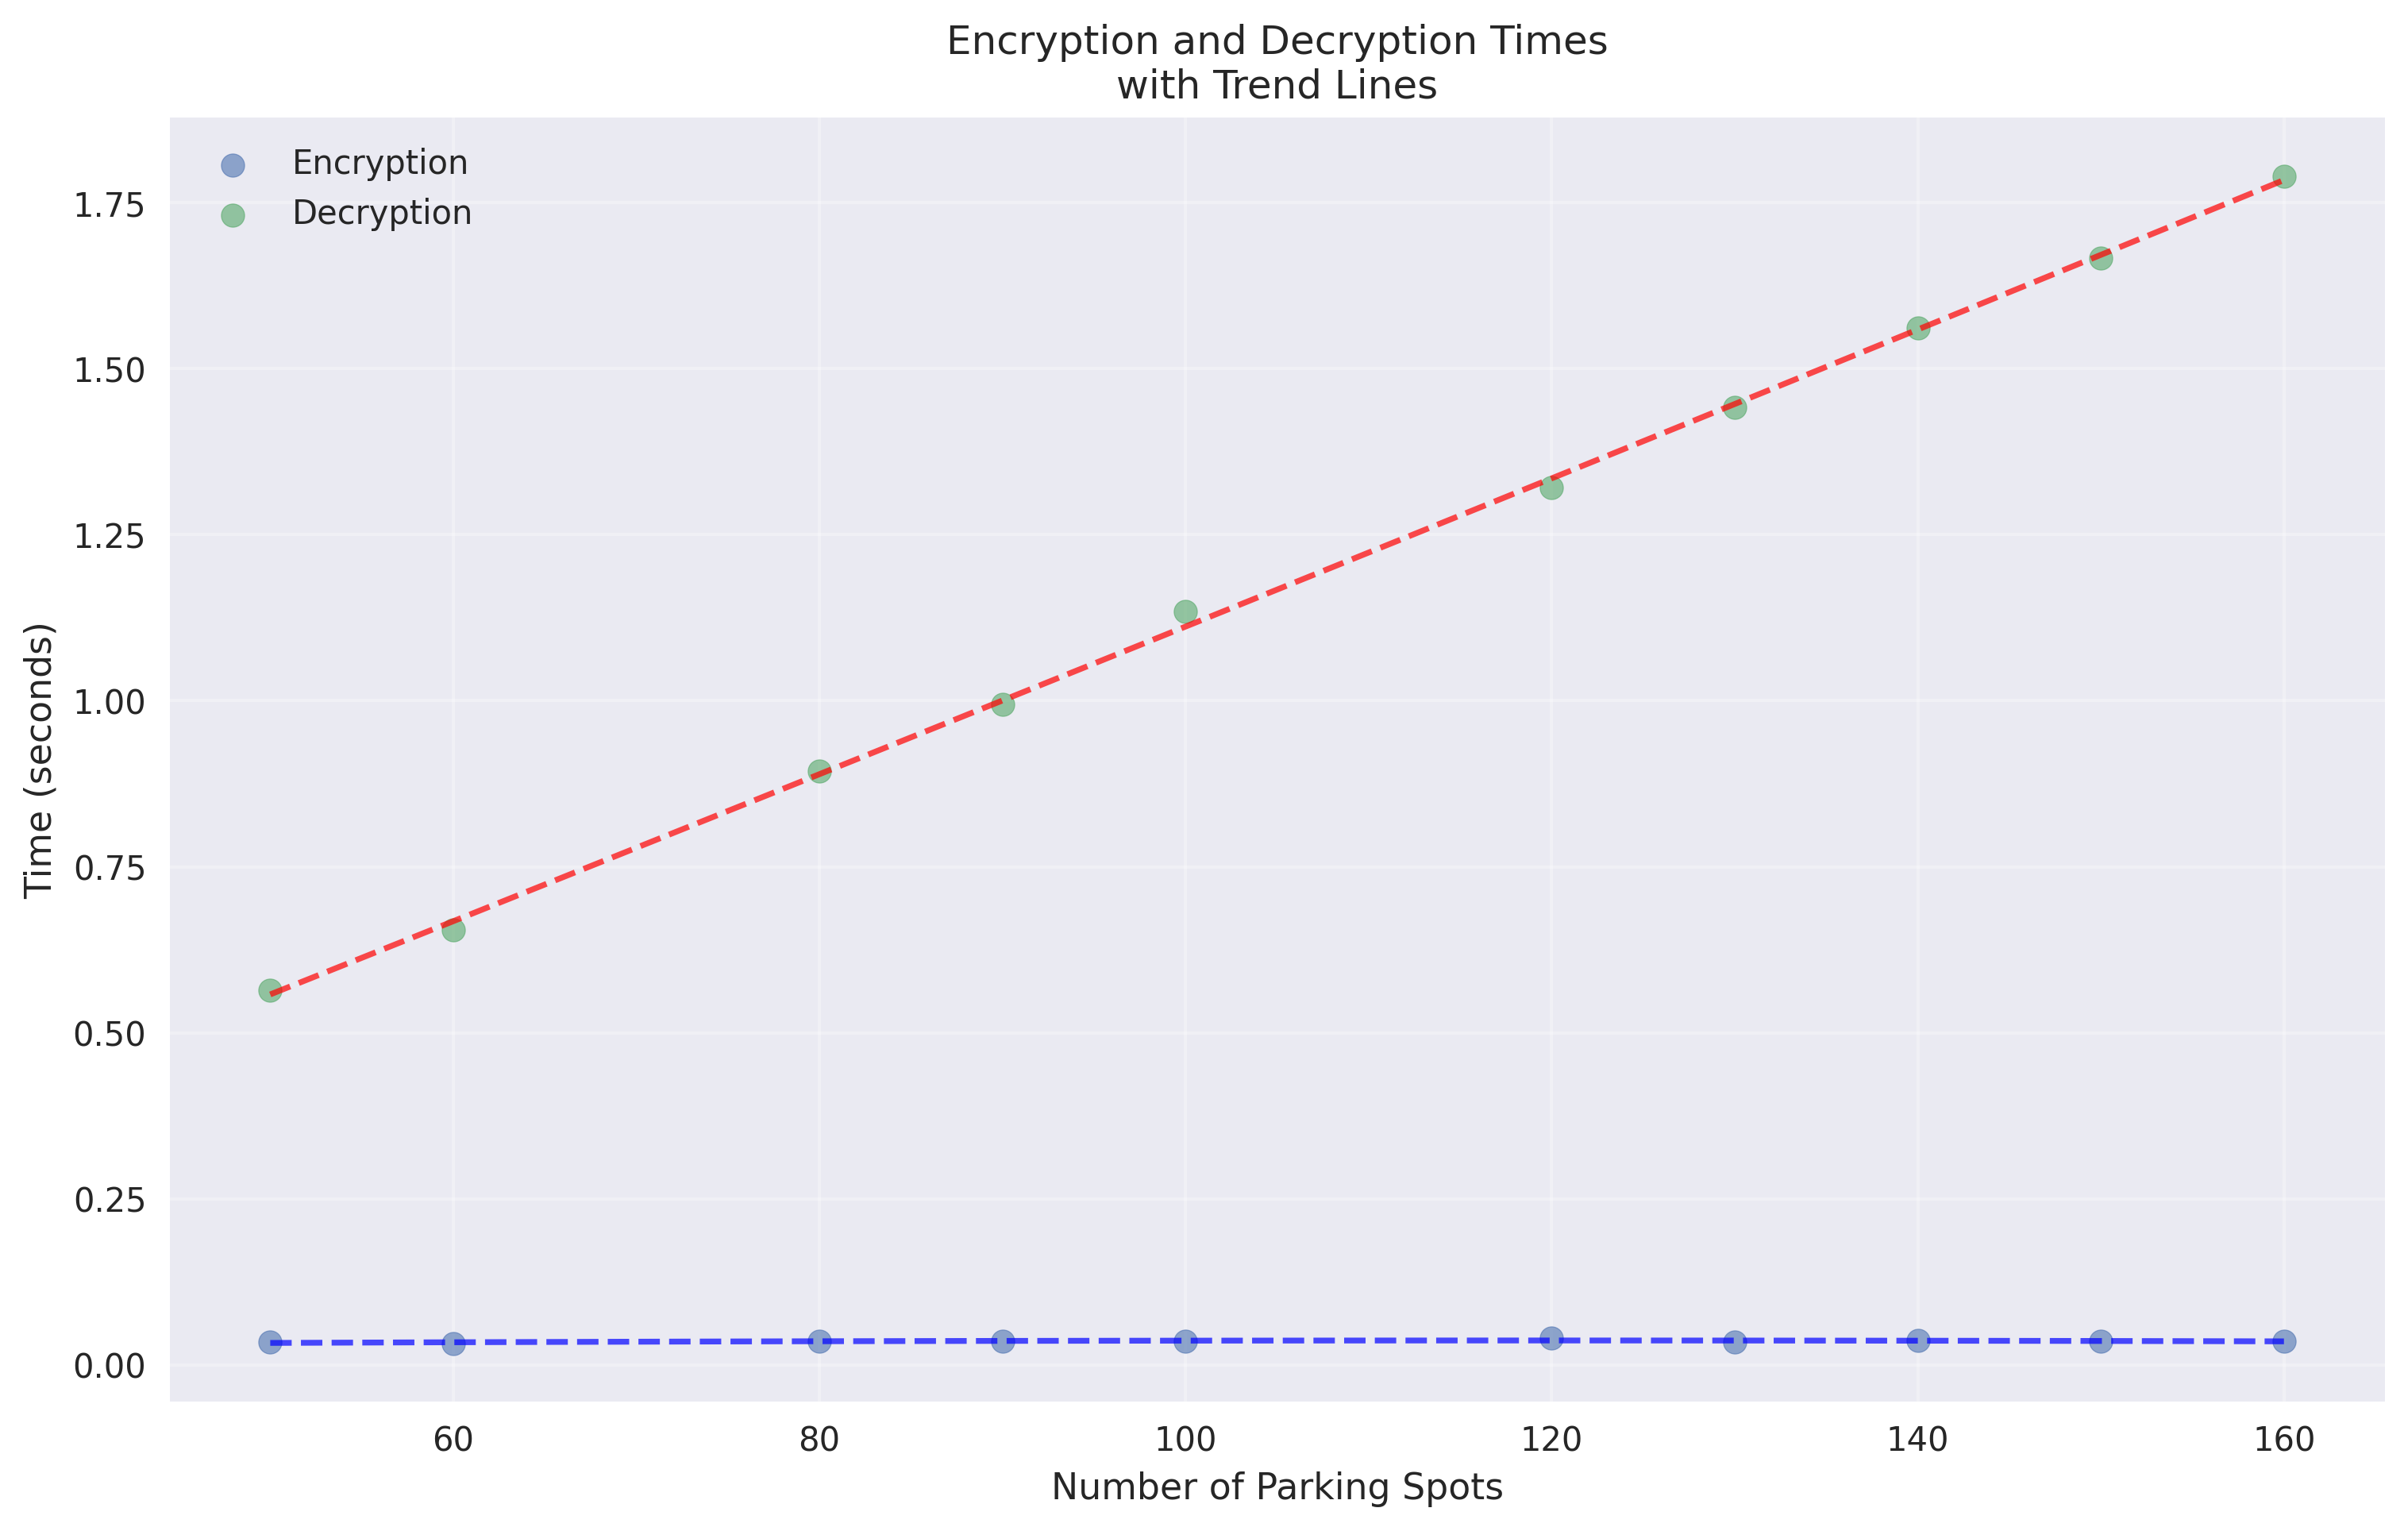
\includegraphics[width=\columnwidth]{img/crypto_times.png}
    \caption{Visualization of the Encryption and Decryption time using HE}
    \label{fig:testing-enc}
\end{figure}

The test begins with the generation of the parameters for the homomorphic encryption scheme, followed by the key generation. The code snippet in Listing \ref{lst:enc-decrypt} shows the code used to encrypt and decrypt the client position.
% add the code to encrypt
\lstset{frame=tb,
  language=python,
  aboveskip=3mm,
  belowskip=3mm,
  showstringspaces=false,
  columns=flexible,
  basicstyle={\small\ttfamily},
  numbers=none,
  numberstyle=\tiny\color{gray},
  keywordstyle=\color{blue},
  commentstyle=\color{dkgreen},
  stringstyle=\color{magenta},
  breaklines=true,
  breakatwhitespace=true,
  tabsize=3
}

\newpage

\begin{lstlisting}[language=python, caption={Encryption and Decryption of the client position}, label={lst:enc-decrypt}]
parameters = CCParamsBGVRNS()
parameters.SetPlaintextModulus(65537)
parameters.SetMultiplicativeDepth(2)

crypto_context = GenCryptoContext(parameters)
crypto_context.Enable(PKESchemeFeature.PKE)
crypto_context.Enable(PKESchemeFeature.KEYSWITCH)
crypto_context.Enable(PKESchemeFeature.LEVELEDSHE)

keypair = crypto_context.KeyGen()
crypto_context.EvalMultKeyGen(keypair.secretKey)
\end{lstlisting}


The next step is to compute the distances between the client position and the parking spots. The code snippet in \cref{lst:compute-distances} shows the code used to compute the distances using the homomorphic encryption scheme.

\begin{lstlisting}[caption={Computing distances using Homomorphic Encryption}, label={lst:compute-distances}]
# Encrypt the client position
query_plaintext = crypto_context.MakePackedPlaintext([query_encoded])
query_ciphertext = crypto_context.Encrypt(keypair.publicKey, query_plaintext)

# Process each spot
spots = parking_system.get_spots()

for spot_id, spot in spots.items():
    # Create plaintext for the spot's encoded position
    spot_plaintext = crypto_context.MakePackedPlaintext([spot['encoded_pos']])
    
    # Homomorphic subtraction to check if positions match
    diff_ciphertext = crypto_context.EvalSub(query_ciphertext, spot_plaintext)
                
    diff_plaintext = crypto_context.Decrypt(keypair.secretKey, diff_ciphertext)

\end{lstlisting}

This two sections from the original codebase showcase how the encryption distance calculation works. The full code contains additional logic for handling metrics and logging.

In order to have a fair comparison with other common encryption standards, I made the test run in parallel by multi-processing on the same machine. This refiniment made the test more realistic, as in a real-world scenario, multiple clients would be sending requests to the server at the same time with multiple parking spots (subscribers).

\begin{figure}[h]
    \centering
    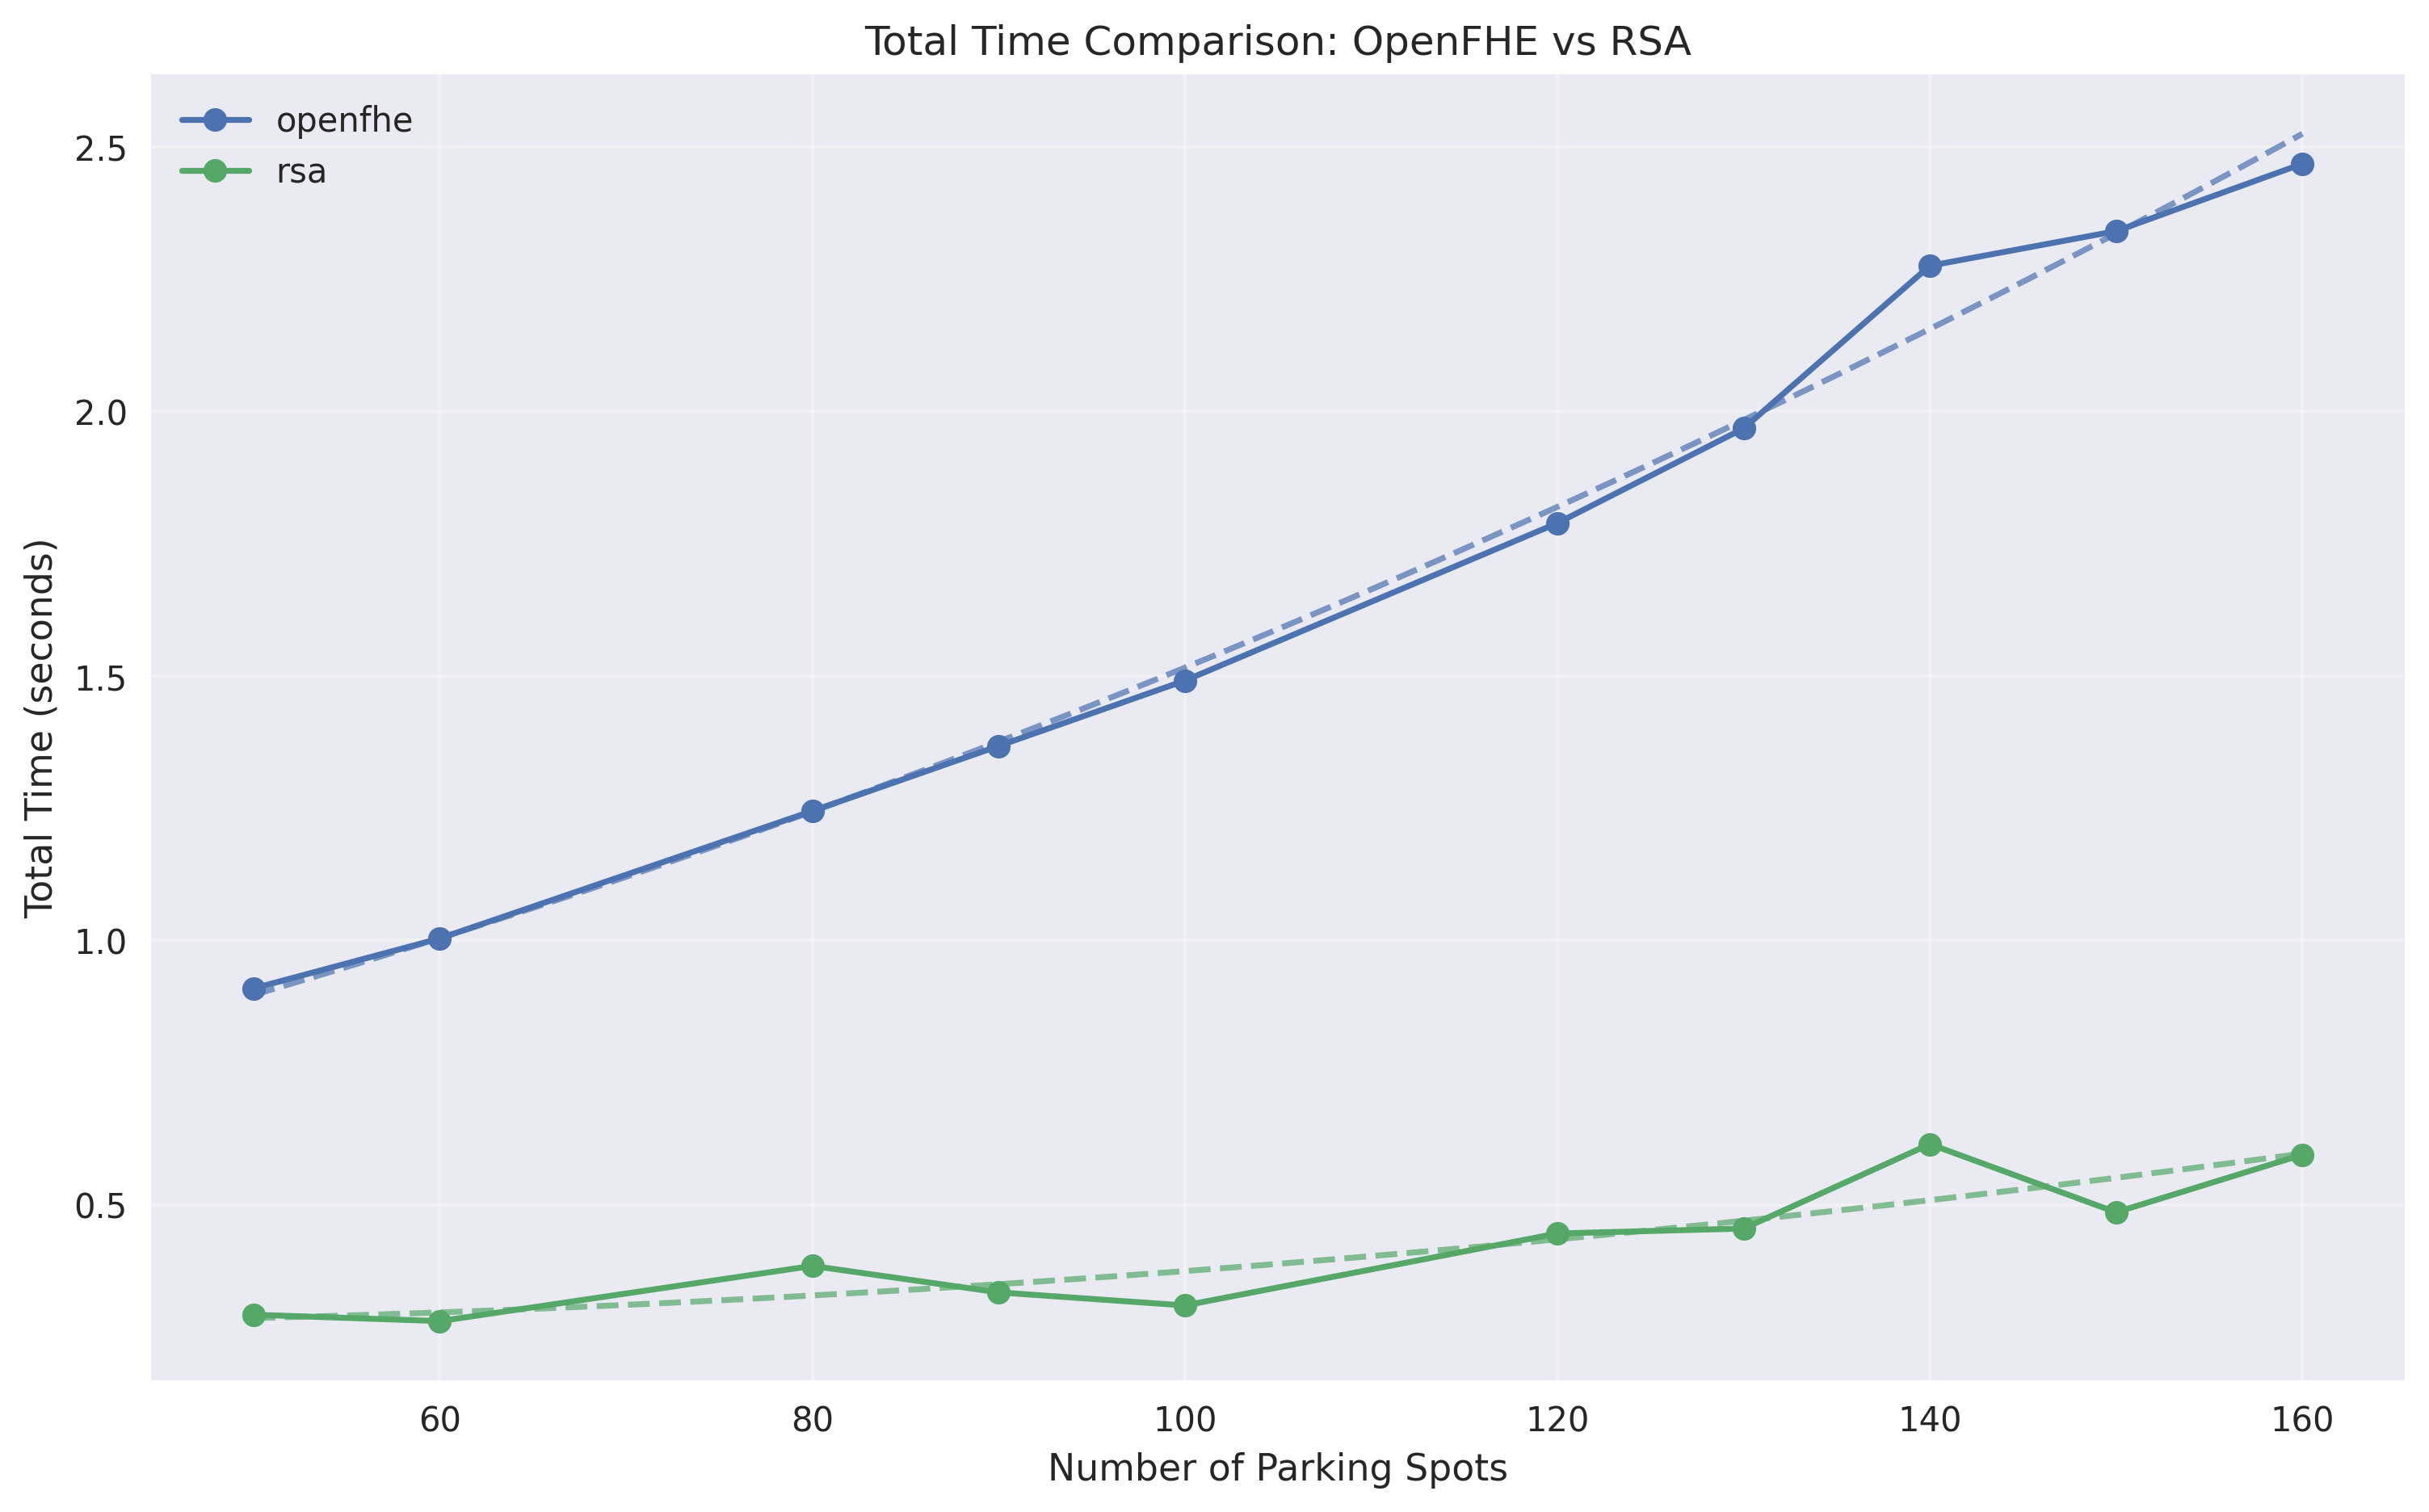
\includegraphics[width=12.5cm,height=9cm]{img/total_time_comparison.png}
    \caption{Comparison between RSA and HE for encryption and decryption}
    \label{fig:he-vs-rsa}
\end{figure}

The overall time performance of the protocol is shown in \cref{fig:he-vs-rsa} confirms that the HE standard has some overhead compared to the RSA standard, but it is still acceptable for a real-world scenario. The main difference between the two encryption standards is that, with the symmetric encryption, the server, after decrypting the client position, is much faster in computing the distances, as it can be achieved in a couple of instructions.

Although the homomorphic encryption needs to perform a simple subtraction, it is still slower, as values need to be packed to match HE standards as done in \cref{lst:compute-distances}.

It also worth to mention the way the distances are computed in our protocol. Firstly, we need to encode the GPS coordinates into a grid-like structure. This operation is essential to ensure that we are considering small areas instead of points \cref{lst:distance-computation}. Then we apply a unique encoding to the grid coordinates, transforming them from a two-dimensional grid into a one-dimensional z-order curve. By having a single integer representation we can perform easily the distance.

\begin{lstlisting}[caption={Distance computation using z-order encoding}, label={lst:distance-computation}]
def calculate_grid_sizes_for_radius(radius_meters, max_lat, min_lat, max_lon, min_lon):
    radius_km = radius_meters / 1000.0
    lat_span = max_lat - min_lat
    lon_span = max_lon - min_lon
    
    # Latitude: fixed ~111.32 km/degree
    lat_cells = int(lat_span / (radius_km / 111.32))
    
    # Longitude: depends on latitude
    mean_lat = math.radians((max_lat + min_lat) / 2)
    lon_cells = int(lon_span / (radius_km / (111.32 * math.cos(mean_lat))))
    
    return lat_cells, lon_cells  # Return separate sizes

def normalize_gps(lat, lon, lat_cells=None, lon_cells=None, edge_meters=500, max_lat=44.499194, min_lat=44.492307, max_lon=11.363250, min_lon=11.325319):

    if lat_cells is None or lon_cells is None:
        lat_cells, lon_cells = calculate_grid_sizes_for_radius(edge_meters, max_lat, min_lat, max_lon, min_lon)
    
    grid_x = int((lat - min_lat) / (max_lat - min_lat) * lat_cells)
    grid_y = int((lon - min_lon) / (max_lon - min_lon) * lon_cells)
    
    return grid_x, grid_y
\end{lstlisting}

To compute the z-order encoding, we use a straightforward approach that interleaves the bits of the x and y coordinates. The code snippet in Listing \ref{lst:z-order-encoding} shows how we compute the z-order encoding for the grid coordinates.

\begin{lstlisting}[caption={Z-order encoding for grid coordinates}, label={lst:z-order-encoding}]
def interleave_bits(x, y):
    """
    Interleave the bits of x and y to create a Morton code.
    x and y should be non-negative integers, each limited to 16 bits.
    """
    # Ensure inputs are within 16-bit range
    x = min(x, 0xFFFF)
    y = min(y, 0xFFFF)
    
    # Convert to binary and pad with zeros to 16 bits
    x_bin = format(x, '016b')
    y_bin = format(y, '016b')
    
    # Interleave the bits
    result = ''
    for i in range(16):
        result += x_bin[i] + y_bin[i]
    
    return int(result, 2)
\end{lstlisting}


There are also other approaches to compute distances between two encrypted points\cite{ibarrond2022hedistancetricks}, as mentioned for the methods in \cref{sec:background-distances}:
\begin{itemize}
    \item \textbf{Cosine similarity:} This can be resolved by normalizing the vectors, i.e., $\mathbf{x}' = \mathbf{x} / \|\mathbf{x}\|$ and $\mathbf{y}' = \mathbf{y} / \|\mathbf{y}\|$, encrypting $\mathbf{x}'$ and $\mathbf{y}'$, and then performing a simple scalar product: $\sum_i x'_i y'_i$.
    
    \item \textbf{Euclidean Distance:} would require a square root operation.\\
    Instead we use the \textbf{Squared Euclidean Distance} instead:
    $
    \mathrm{SED}(\mathbf{x}, \mathbf{y}) = \sum_i (x_i - y_i)^2
    $
    
    \item \textbf{Manhattan Distance:} in this case it is also require computing the absolute value.\\
    If you encrypt only binary values (i.e., $\hat{\mathbf{x}}, \hat{\mathbf{y}}$ such that $\hat{x}_i, \hat{y}_i \in \{0,1\}$ for all $i$), you can reformulate:
    $
    \mathrm{MD}(\hat{\mathbf{x}}, \hat{\mathbf{y}}) = \sum_i (\hat{x}_i - \hat{y}_i)^2 = \mathrm{HD}(\hat{\mathbf{x}}, \hat{\mathbf{y}})
    $
    which is the \textbf{Hamming Distance} . For non-binary vectors, you can at least compute the \textbf{Squared Manhattan Distance}
    $
    \mathrm{SMD}(\mathbf{x}, \mathbf{y}) = \sum_i (x_i - y_i)^2
    $
    but this is missing a square root to recover the standard Manhattan distance.
    
\end{itemize}

Rounding off, all of these methods have the problems of relying on calculations on floating point numbers, which is not ideal for homomorphic encryption. Another way could be to normalize the coordinates to integers, with a fixed order of magnitude, but it is not worth the effort, as the z-order encoding is already a good solution for this problem.



\section{Conclusions and Future Works}

From the testing phase, we can conclude that the protocol is feasible and functional. The performance of the homomorphic encryption scheme is acceptable for a real-world scenario, although it is still computationally more expensive than a traditional RSA solution. However, it can be applied in a zero-trust scenario, where the server cannot be trusted to handle sensitive data. The introduction of PRE (Proxy Re-Encryption) allows us to offload the computation to a trusted third party, which can be used to compute the distances between the client position and the parking spots without revealing the client position to the server. Moreover, this resolved the previous issue of the server possible leak of client position, under the threat model~\cref{subsec:threatmodel}.

One more factor to consider is the scalability of the protocol. The MCs and LDs can be scaled horizontally, meaning that we can add more servers to handle more clients and parking spots. The same applies to the server and workers; for instance, we can have multiple servers handling different areas of the metropolis, each with its own set of parking spots. However, the CA (Certificate Authority) is not. Moreover, the CA could have multiple instances, but they would need to be synchronized in order to issue certificates for the same client.

During the testing phase, we identified several areas for improvement for future work. One of them is the possible integration of IoT specific libraries, such as the \emph{SEAL Embedded} \cite{sealembedded} library, which is designed for resource-constrained devices. This would allow us to run the protocol on edge devices, such as sensors or micro-controllers, without the need for a powerful server. The obvious constraint is that the whole system should be adapted to work with the Microsoft SEAL\cite{sealcrypto} Library also on the server side. 

Another huge area of possible optimization is the adjacency calculation using z-order encoding and FHE. In the paper \cite{zhang2020privacy}, they proposed a standard for computing useful queries on homomorphic encrypted position-related data. In their work, they were considering a social media application, that was collecting user positions to show nearby friends. Their work not only showcased that you can apply z-order encoding to encode positions, but comes really handy when using preference levels for positions sharing. Let's consider the following example: a user wants to share his position with a friend, but he knows that that friend is not trusted enough to share his exact location. Instead, he can apply a preference bit-mask in order to share only a certain order level of the z-order encoding. The paper also shows that is possible to compute the exact distance between two positions: the main idea is to create the smallest encoded box that contains both positions. This concept could be applied to our protocol, allowing us not only to find parkings sharing our same area, but also to compute the distance between a particular parking.


Our encoding standard is based on the transformation of GPS coordinates into a z-order curve, thus an approximate representation of an area. When applying this encoding, we need to consider the order of magnitude of the error introduced by the encoding. That doesn't always mean that the error is negligible, but at the same time could also work in our favor, as it allows to obfuscate an exact position.

In conclusion, the protocol presented in this thesis is a feasible solution for the problem of finding nearby parking spots in a zero-trust scenario. This was possible thanks to the correct usage of the right network protocols, such as the publish/subscribe and request/response protocols. During my work, I concluded that even though the publish/subscribe protocol is preferred for this kind of applications, it does not match the requirements of a zero-trust scenario. Moreover, working with homomorphic encryption adds the requirement that the server is not allowed to know the plain text of the clients. This is a crucial point, as it does not allow us to infer informations from the client data. So, the request/response protocol works better in this sense: the client request anonymously a service, the server responds applying a list of operations to the encrypted data, and then the client can decrypt the result. In the opposite case, the server would need to know \emph{when} to respond to the client, which is most of the time a consequence of a side-effect to the request. Let's consider the case the LA-MQTT protocol \ref{sec:la-mqtt}: the client subscribes to a topic, and the server publishes the result based on the client location. In this case, is obvious that the server needs to know the client position in order to publish the result. Indeed, if this was the case, we would not be able to apply the homomorphic encryption scheme.


\renewcommand{\bibsection}{}
\chapter*{References}
\bibliography{refs}
\newpage

\renewcommand{\appendixtocname}{Appendices}
% \csname @openrightfalse\endcsname
\pagenumbering{gobble}

\newpage~\newpage
\chapter*{Ringraziamenti}
Grazie a tutti
\end{document}
